\section{刘学州事件的完整研究}

仓库里“\texttt{刘学州-评论-情感演化分析-BERT}”有一百七十二个节点，从五份评论 CSV 做到论文里的图和表。
不必照抄全部，看懂它怎么分段就够了：先做一份干净总表，再在总表上派生指标，最后把同一个套路复制到五个阶段。

\subsection{第一段\quad 合并与清洗}

最左边五个上传节点各挂一份评论 CSV，汇到一个输出节点合并成总表。后面接清洗、筛选保留行、归一化去重、近重复去重四步。
每一步都留一个输出节点，中间结果随时能翻出来对账，出问题能定位到具体哪一步把行弄丢了。

\begin{figure}[H]\centering
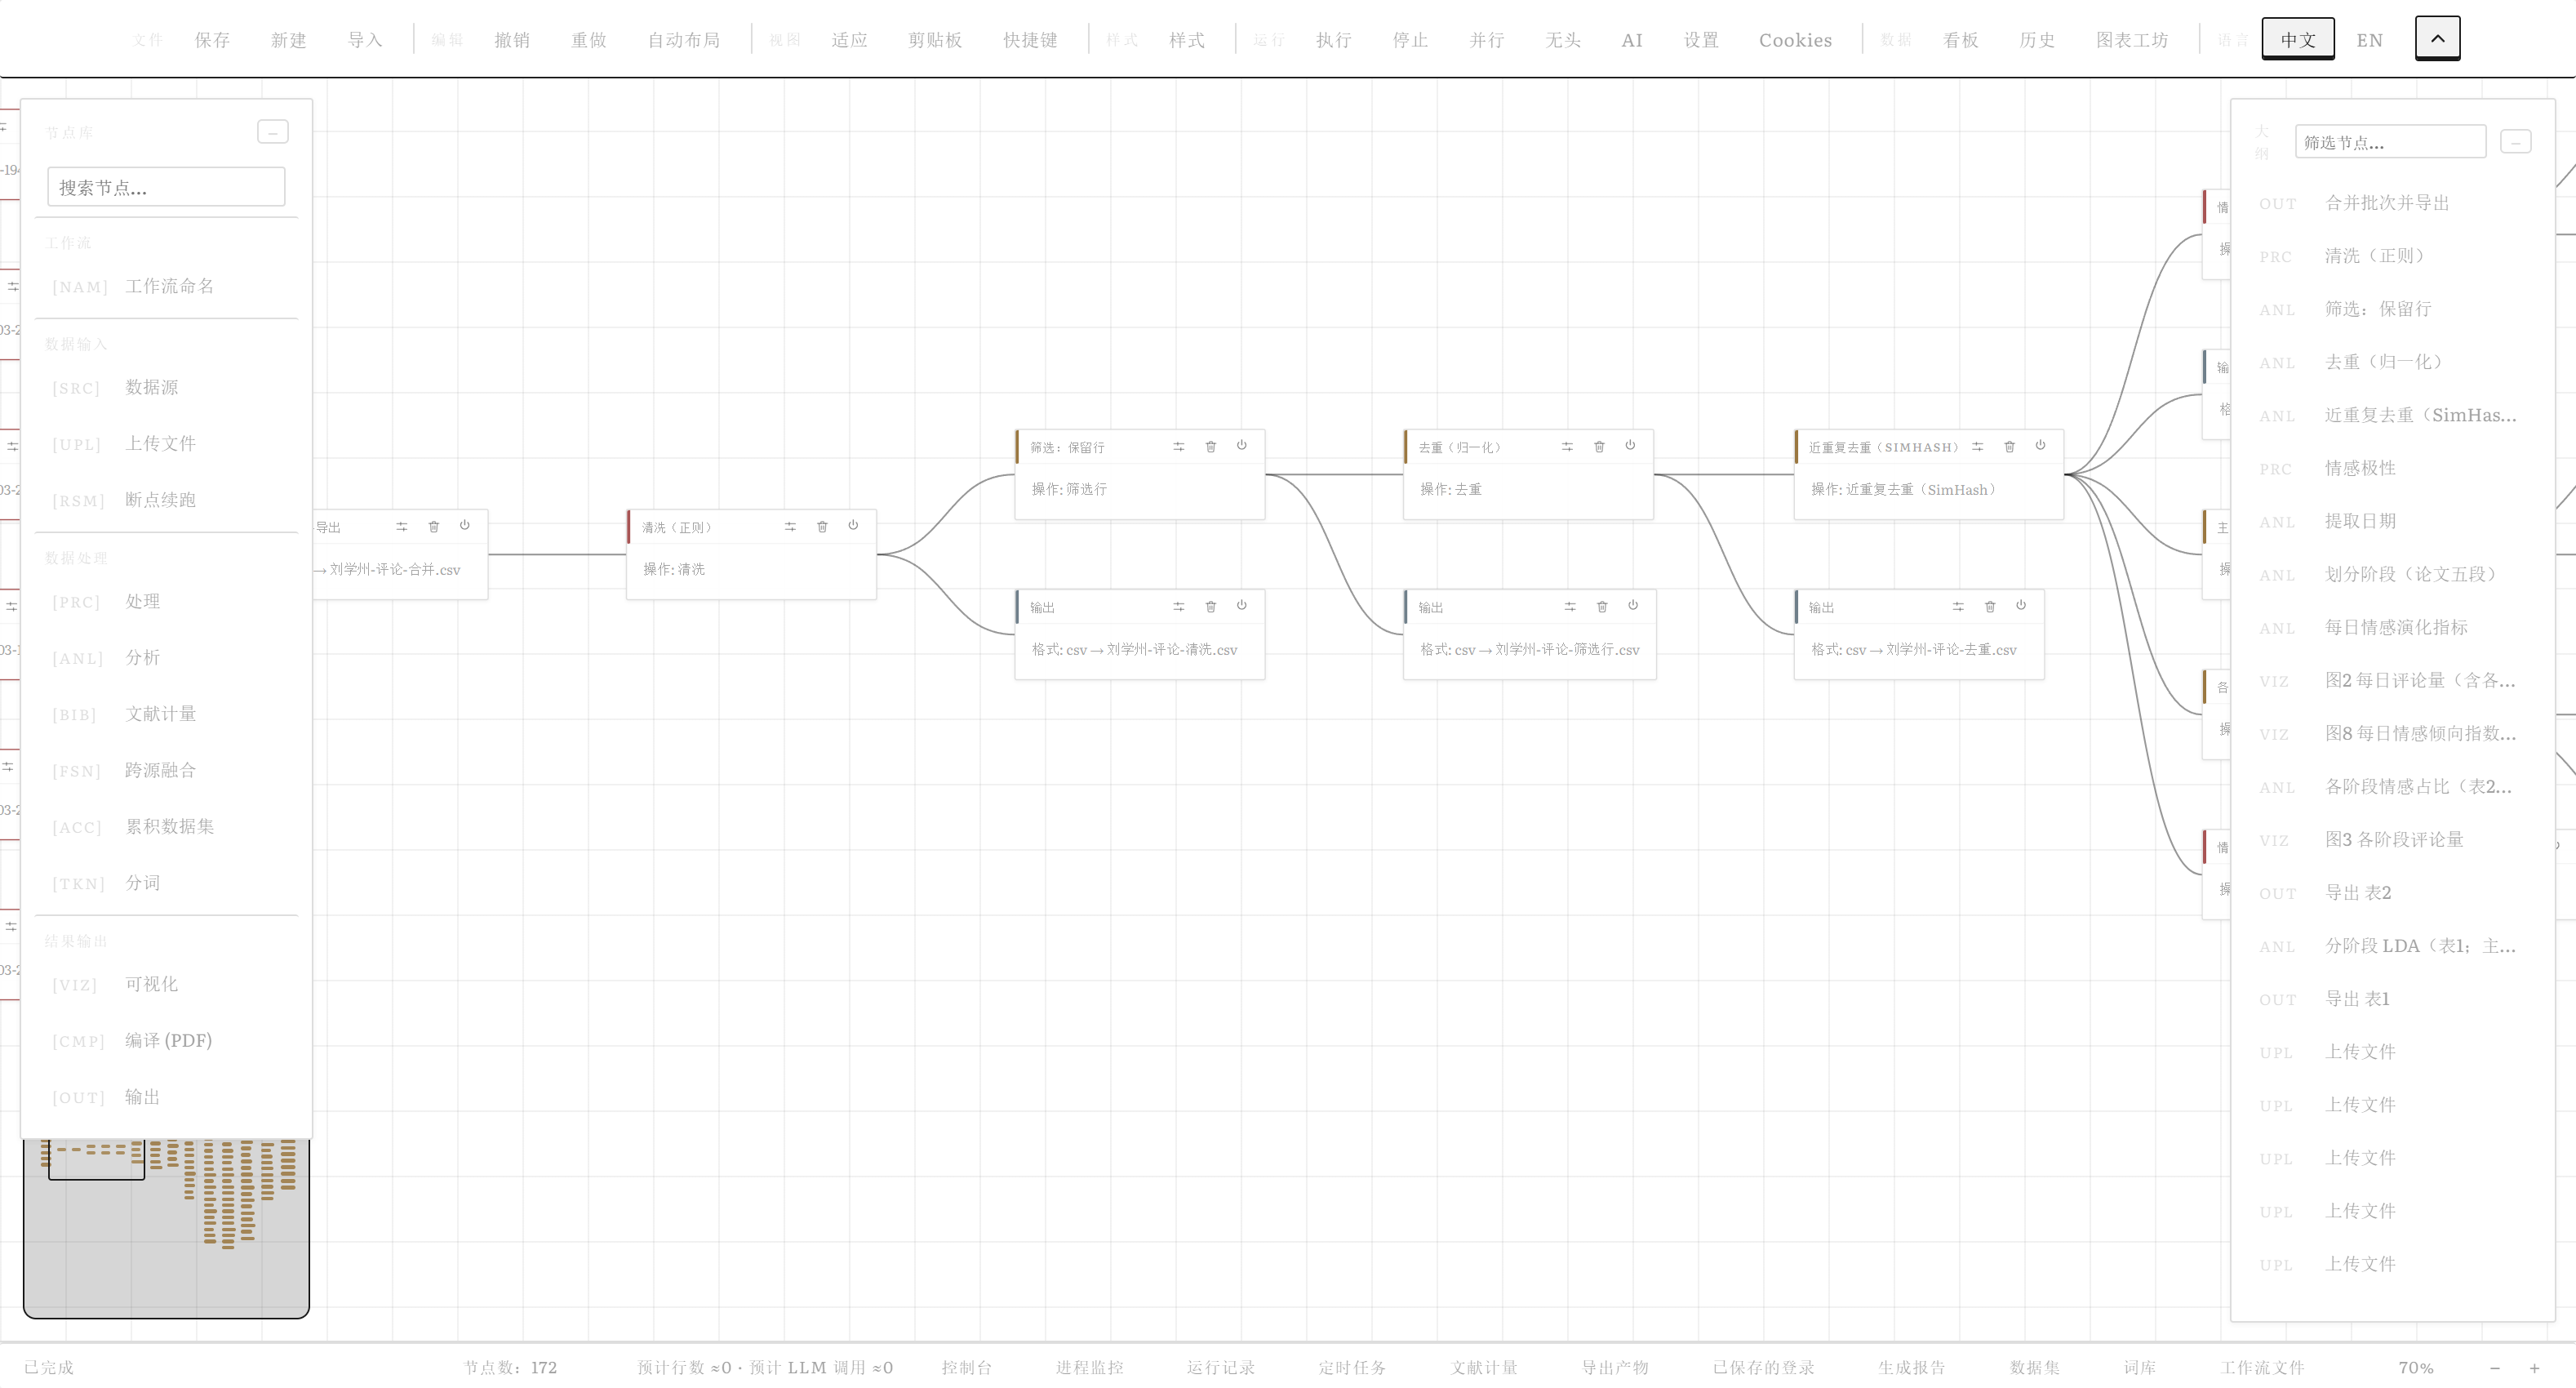
\includegraphics[width=0.98\textwidth]{liu-zoom-clean.png}
\caption{合并、清洗、三层去重，每一步都留一份 CSV 对账}
\label{fig:liu-clean}
\end{figure}

\subsection{第二段\quad 打分与分阶段}

情感极性用微调模型整列推理，正负阈值 0.6 与 0.4，结果写进标签与分数两列。接着提取日期，按六条边界切出五个阶段，
阶段序号一并写出来。阶段边界来自论文，不是程序猜的；想自己定边界时，先用建议边界那个算子看曲线。

\begin{figure}[H]\centering
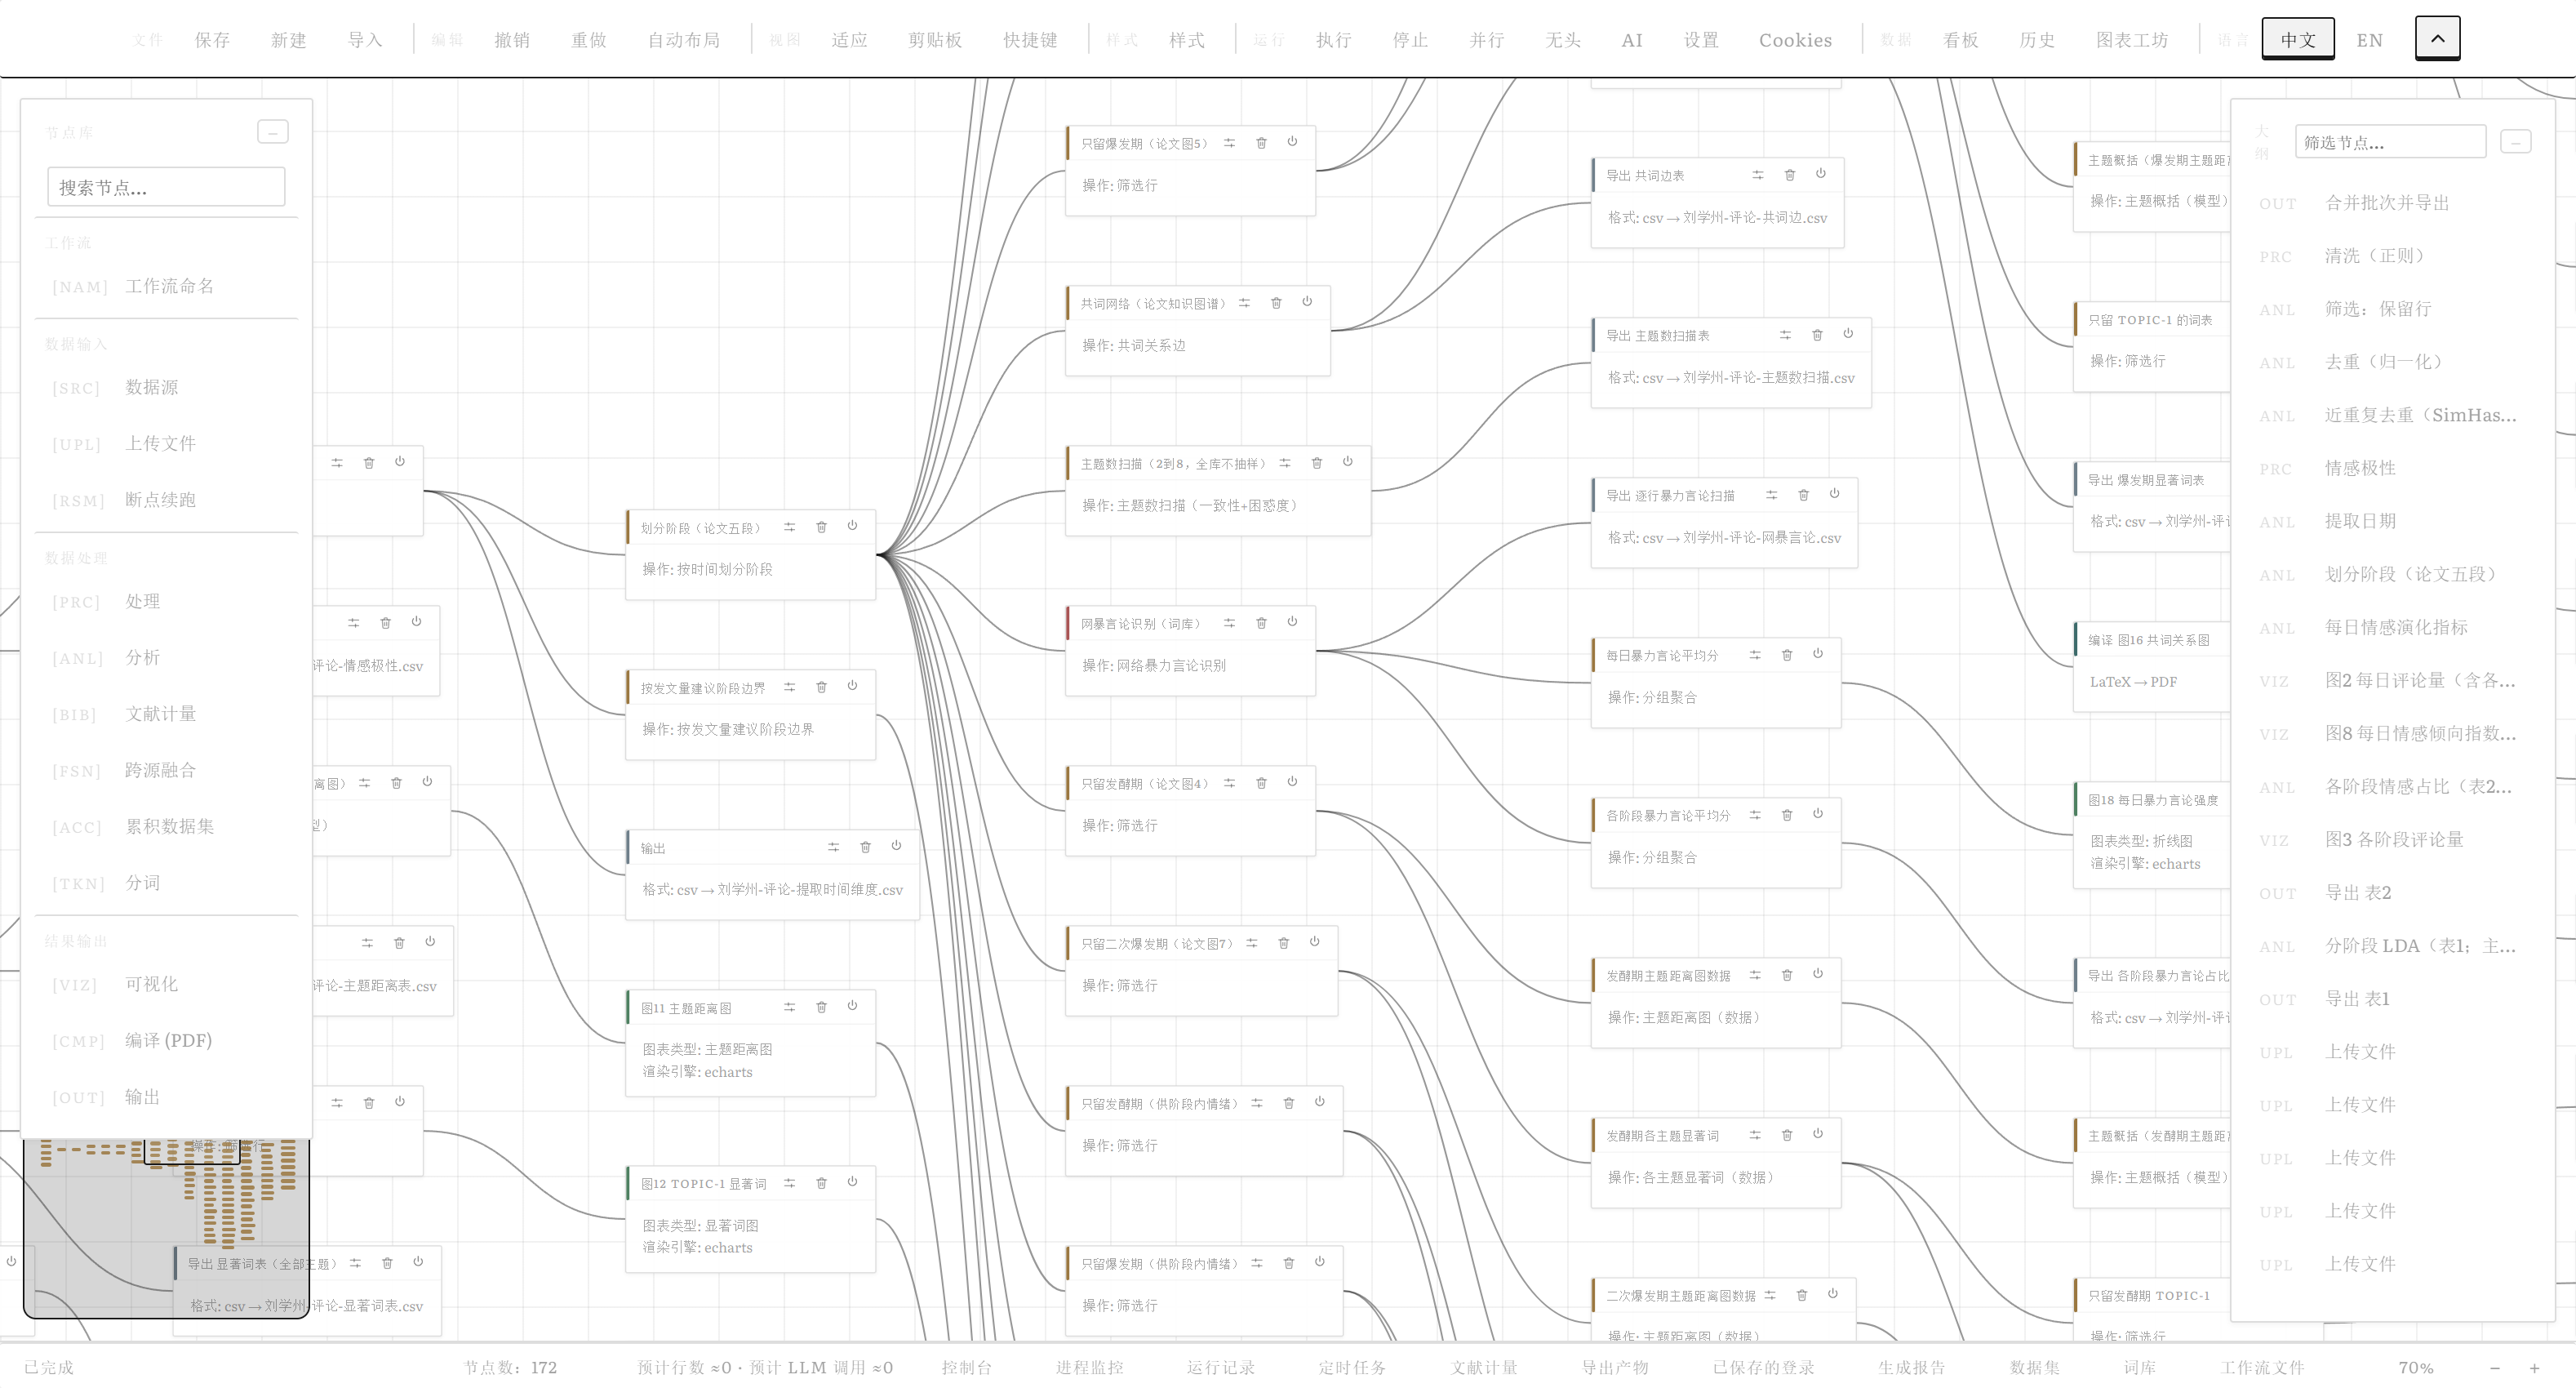
\includegraphics[width=0.98\textwidth]{liu-zoom-stage.png}
\caption{划分阶段把一张总表分成五个分支，每个分支一套主题与情感图}
\label{fig:liu-stage-branch}
\end{figure}

\subsection{第三段\quad 主线的四张图}

每日评论量、每日情感指数、各阶段评论量、各阶段情感占比，四张图构成主线的证据。每日评论量那张带事件标注，
几个峰值日上画竖虚线并写一句话，标注的位置必须与横轴取值一字不差，对不上会拒绝并列出可选值。

\subsection{第四段\quad 主题}

分阶段主题、主题概括、主题距离、显著词、生命周期、流向、共词网络一路做下来。主题距离图用气泡大小表示占比，
标签用概括那一列，不是 Topic-1 这种编号。

\subsection{第五段\quad 预警与攻击性}

情感走向外推与二次爆发预警各一条链。网暴言论识别单独一条，按日期与阶段各聚合一次，得到每日攻击性均值与各阶段对比。

\subsection{第六段\quad 分阶段复制}

同一个套路在五个阶段各复制一遍，每段有自己的主题图、显著词、阶段内情感曲线。节点多，但结构重复，学会一段就会五段。
中间任何一步都能单独重跑，下游自动复用没变的部分。

\subsection{这条工作流教了什么}

三段式。先做一份干净的总表，再在总表上派生各种指标，最后复制成图。长链的关键步骤都留一个输出节点，
每个阶段的结论都能落成文件，论文里的每个数字都能顺着文件找回它是哪一次运行、哪一列算出来的。
